\section{Model}

The TMD system is described by
the effective tight-biding, low-energy, two-valley Hamiltonian
\cite{PhysRevLett.108.196802},
\begin{equation}
  \label{eq:tmd:hamiltonian}
  H_τ^0 \ofK
  = a t \left( τ k_x σ_x + k_y σ_y \right) ⊗ I_2
    + \frac{Δ}{2} σ_z ⊗ I_2 - λ τ \left(σ_z - 1 \right) ⊗ S_z.
\end{equation}
The (periodic) Bloch orbital states
(see \cref{s:appendix:tight-binding}) are
\begin{equation}
  \ketOrbitalK{ν}
  = \frac{T_{\vK +  τ \vc{K}}}{\sqrt{N}}
    ∑_{n = 1}^N e^{i \left( \vK + τ \vc{K} \right) ⋅ \vRn{n}}
    T \of{\vRn{n}} \ketOrbital{ν},
\end{equation}
where $N$ is the number of \ce{M}-type atoms in the system,
\begin{subequations}
  \begin{alignat}{2}
    & \ketOrbital{+} && = \Ket{d_{z^2}} ⊗ \Ket{\s}, \\
    & \ketOrbital{-} && = \frac{1}{\sqrt{2}}
        \left( \Ket{d_{x^2 - y^2}} + i τ \Ket{d_{xy}} \right) ⊗ \Ket{\s},
  \end{alignat}
\end{subequations}
and $\Ket{d_{xy}}$ and $\Ket{d_{x^2 - y^2}}$
refer to the angular momentum orbitals
in the symmetry group $E \left( d_{xy}, d_{x^2 - y^2} \right)$.
The operators $σ_i$ are Pauli operators acting
on the two Bloch orbital states
(indexed by $ν = ±$)
such that $σ_z \ketOrb{±}{\ofK} = ± \ketOrb{±}{\ofK}$.
The valley index $τ = ±$, corresponding to the $± \vc{K}$ points,
and the spin index ${\s} = ±$ (or ${\s} =\ ↑↓$),
corresponding to the $z$-component of the spin through $s_z = {\s} / 2$,
are good quantum numbers.
The momentum $\vK$ is measured from the valley center,
i.e., for a given valley, the total momentum relative to the center
of the Brillouin zone is $\vK + τ \vc{K}$.
The energy gap is $Δ$, the spin splitting in the valence band is $2 λ$,
the lattice constant is $a$, and $t$ is the effective hopping integral.
\Cref{eq:tmd:hamiltonian}
can be written in matrix form in the Bloch orbital basis,
\begin{equation}
  \left[ H_{τ σ}^0 \ofK \right]
  = \left[
    \begin{matrix}
      \dfrac{Δ}{2}                     & a t \left( τ k_x - i k_y \right) \\
      a t \left( τ k_x + i k_y \right) & λ τ \s - \dfrac{Δ}{2}
    \end{matrix}
    \right].
\end{equation}

The energy spectrum,
\begin{equation}
  \label{eq:energy}
  \fnEnergy{n} \of{k}
  = \frac{1}{2} \left( λ τ {\s} + n \sqrt{{\left( 2 a t k \right)}^2
  + {\left( Δ - λ τ {\s} \right)}^2} \right),
\end{equation}
with $k = \abs{\vK}$
and $n = 1$ ($n = -1$) indexing the conduction (valence) band
is shown in \cref{fig:energy}.
For a fixed band, we have the inverse relation,
\begin{equation}
  {\left( \frac{a t k}{Δ / 2} \right)}^2
  = {\left( \frac{2 E}{Δ} \right)}^2
    + 2 τ σ \left( \frac{λ}{Δ} \right) \left( 1 - \frac{2 E}{Δ} \right) - 1,
\end{equation}
where $E > Δ / 2$ for $n = 1$ and
$E < - \left( Δ / 2 - λ τ σ \right)$ for $n = -1$.
Note the relations
\begin{subequations}
  \begin{align}
    θ_{-↓}^{n} \of{k} + θ_{+↑}^{n} \of{k} & = 2π , \\
    \fnTheta{+} - \fnTheta{-} & = - τ π, \\
    ϕ_{-\vK} - ϕ_{\vK} & = π.
  \end{align}
\end{subequations}

\begin{figure}
  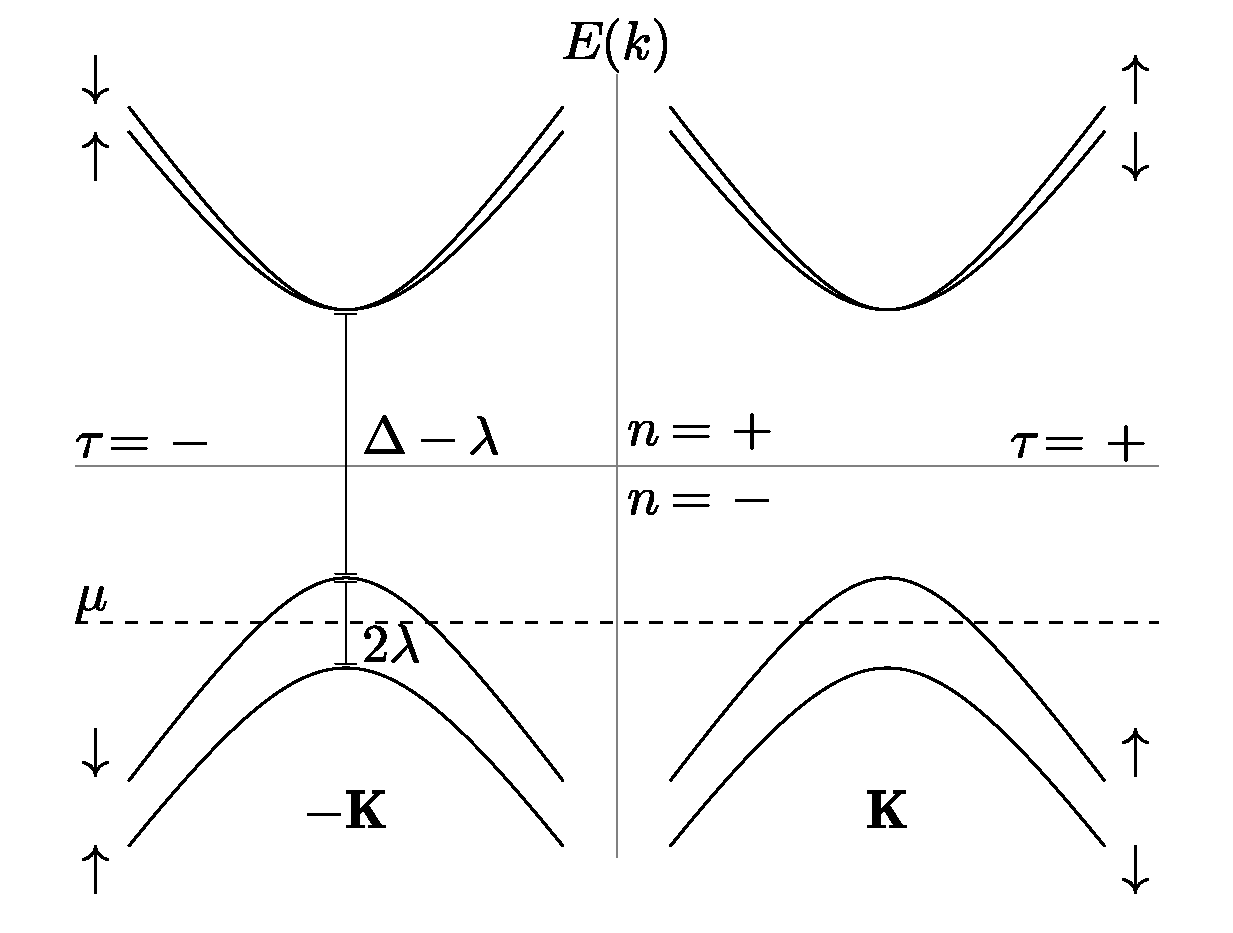
\includegraphics[width=\columnwidth]{figures/energy-bands}
  \caption{%
    Energy bands for $\ce{WSe2}$ as given by \cref{eq:energy}
    with $a t = \SI{3.939}{\electronvolt \per \angstrom}$,
    $Δ = \SI{1.60}{\electronvolt}$,
    and $λ = \SI{0.23}{\electronvolt}$.
    Each valley is centered at $± \vc{K}$ relative to the center of the
    Brillouin zone.
    The energy for a given band depends only on the distance $k$
    measured from the valley center.
  }\label{fig:energy}
\end{figure}

We focus on doped systems
such that the chemical potential $μ$ lies in the upper valence bands.
Within each band, the Bloch basis eigenstates are written
in terms of the orbital states as elements on the Block sphere,
\begin{equation}
  \Ket{u_{τ {\s}}^n \of{k, ϕ}}
  = \cos{\frac{\fnTheta{n}}{2}} \ketOrb{+}{\of{k, ϕ}}
  + e^{-i τ ϕ}
    \sin{\frac{\fnTheta{n}}{2}} \ketOrb{-}{\of{k, ϕ}},
\end{equation}
where $k_x + i τ k_y = k e^{i τ ϕ}$ and
\begin{equation}
  \tan{\frac{\fnTheta{n}}{2}}
  = \frac{a t τ k}{\dfrac{Δ}{2} - \fnEnergy{-n} \of{k}}
  = \frac{a t τ k}{\fnEnergy{n} \of{k} - \fnEnergy{-} \of{0}}.
\end{equation}
The polar angle on the Bloch sphere
of the conduction and valence bands are related by
$\fnTheta{-} - \fnTheta{+} = τ π$.
The mapping of the energy band to the Bloch sphere,
parametrized by $\left( θ, ϕ \right)$,
encodes the topological character:
as one moves from the node out to infinity,
the states sweep either the northern or southern hemisphere
with a chirality determined by the Berry curvature.
